% Wide figures are declared before the running text so the compositor can fill each page.

\begin{figure*}[!tbp]
\begin{minipage}{\textwidth}
\centering
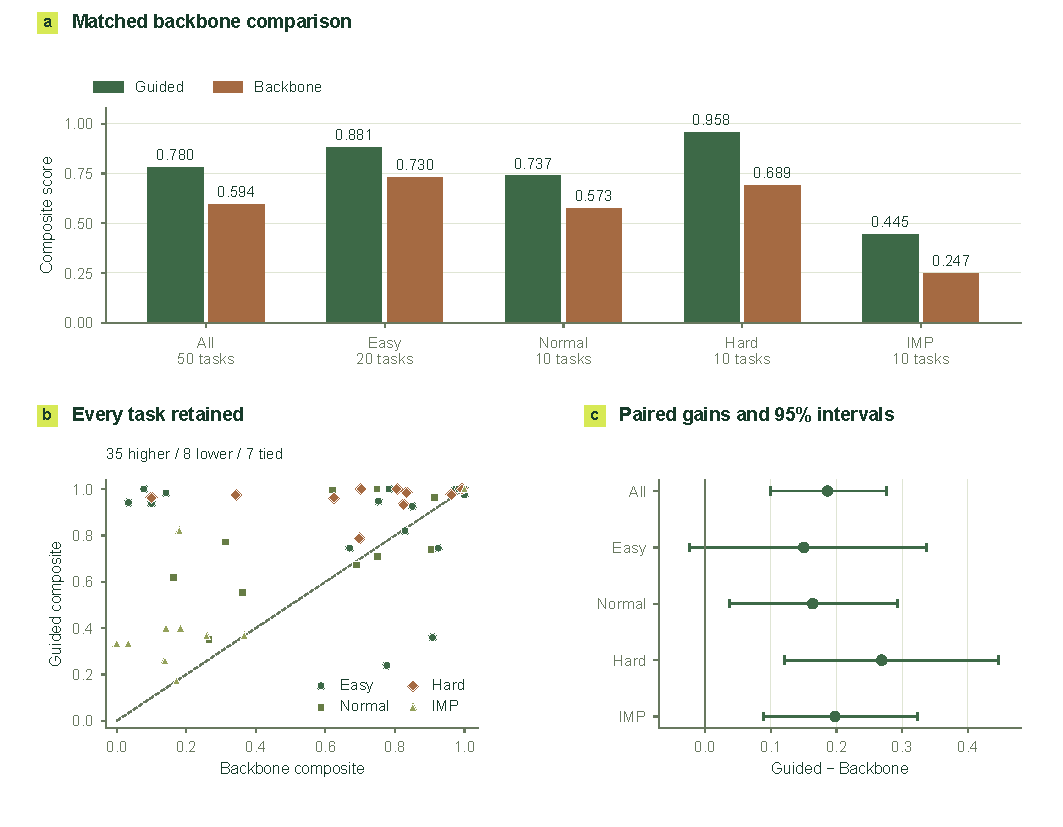
\includegraphics[width=\textwidth]{figures/bench_overview.pdf}
\caption{P2 benchmark outcomes under the archive-adjudicated track. (a) Guided and the same-backbone Standard baseline across all 50 tasks and each tier. (b) All 50 paired task outcomes. (c) Mean paired score differences with 95\% percentile intervals from 100,000 task-level bootstrap resamples. Each task has one run per configuration; Easy contains 20 tasks and the other tiers contain 10 each.}
\label{fig:bench-overview}
\end{minipage}
\end{figure*}

\begin{figure*}[!tbp]
\begin{minipage}{\textwidth}
\centering
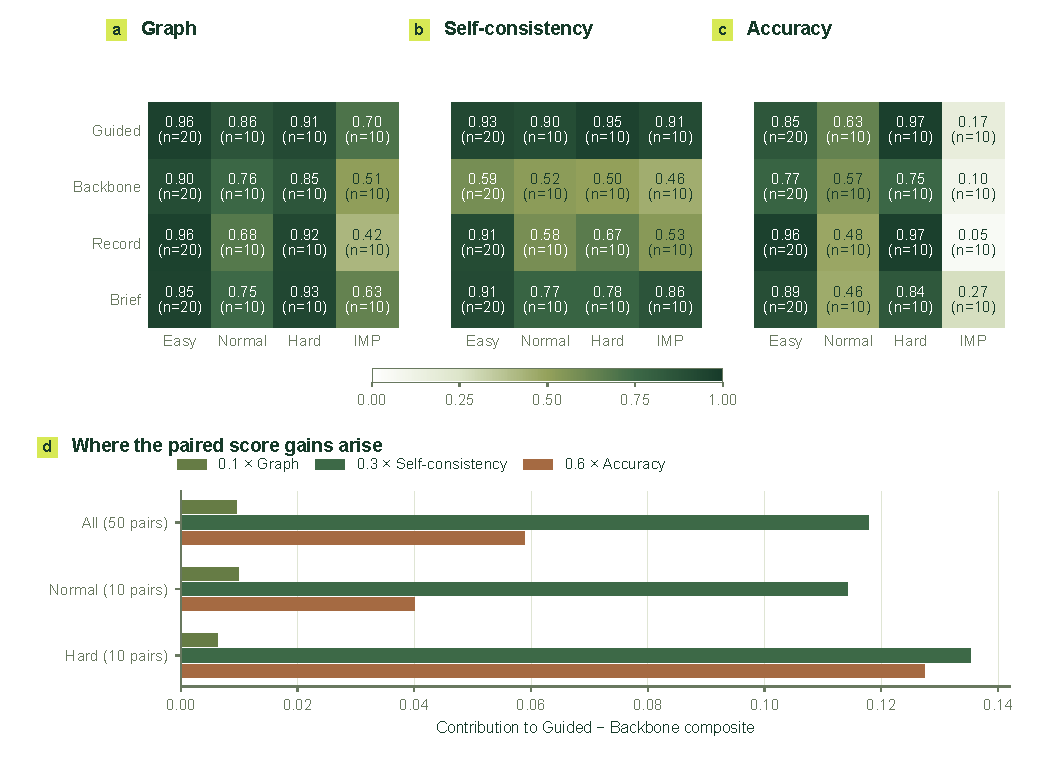
\includegraphics[width=\textwidth]{figures/bench_components.pdf}
\caption{CloudraBench score layers across all 200 organized runs. (a--c) Means of Graph, Self-consistency, and Accuracy in each arm and tier, using 50 tasks per arm overall, 20 Easy tasks, and ten tasks in each other tier. (d) Guided--Backbone mean differences decomposed with the fixed weights 0.1/0.3/0.6, using all 50 pairs, ten Normal pairs, and ten Hard pairs. Components are aligned with the final organized totals using each run's recorded research materials and score records.}
\label{fig:bench-components}
\end{minipage}
\end{figure*}

\begin{figure*}[!tbp]
\begin{minipage}{\textwidth}
\centering
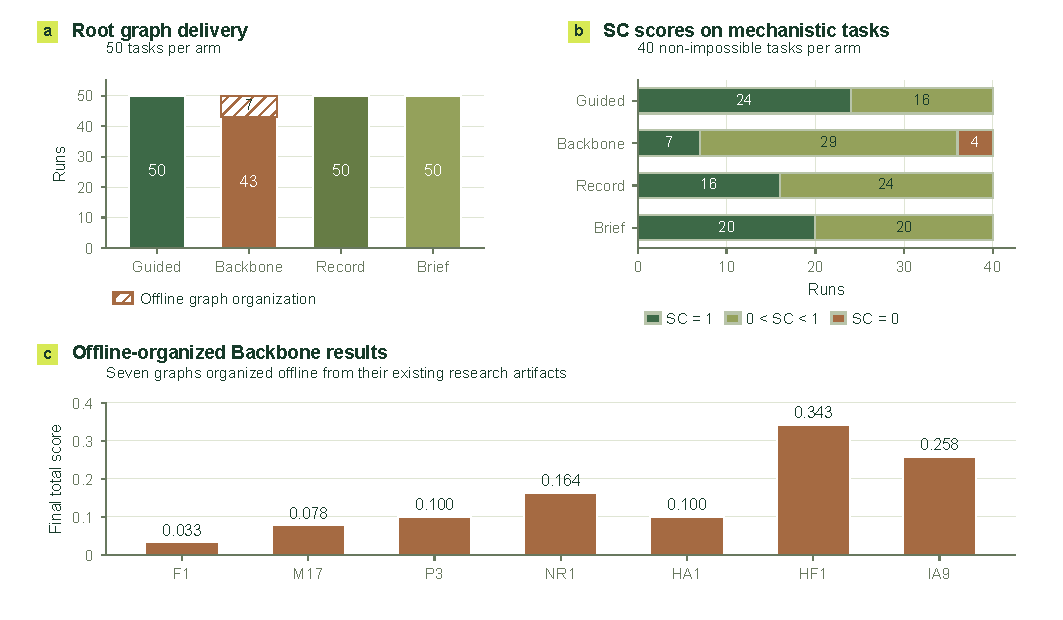
\includegraphics[width=\textwidth]{figures/bench_delivery.pdf}
\caption{Runtime graph delivery and final scientific support in P2. (a) Original root mechanism graphs across 50 tasks per arm: Guided 50, Backbone 43, Record 50, and Brief 50. The hatched segment marks seven additional Backbone graphs assembled offline from the runs' own research materials; the organized set contains 50 graphs per arm. (b) Final continuous self-consistency (SC) scores for all 40 non-Impossible tasks per arm, separating SC = 1, partial positive credit, and SC = 0. Full-score counts are 24, 7, 16, and 20; Backbone has four zero-score tasks. (c) Organized composite scores for the seven Backbone tasks without runtime root graphs, ranging from 0.0333 to 0.3425 (mean 0.1537).}
\label{fig:bench-delivery}
\end{minipage}
\end{figure*}

\begin{figure*}[!tbp]
\begin{minipage}{\textwidth}
\centering
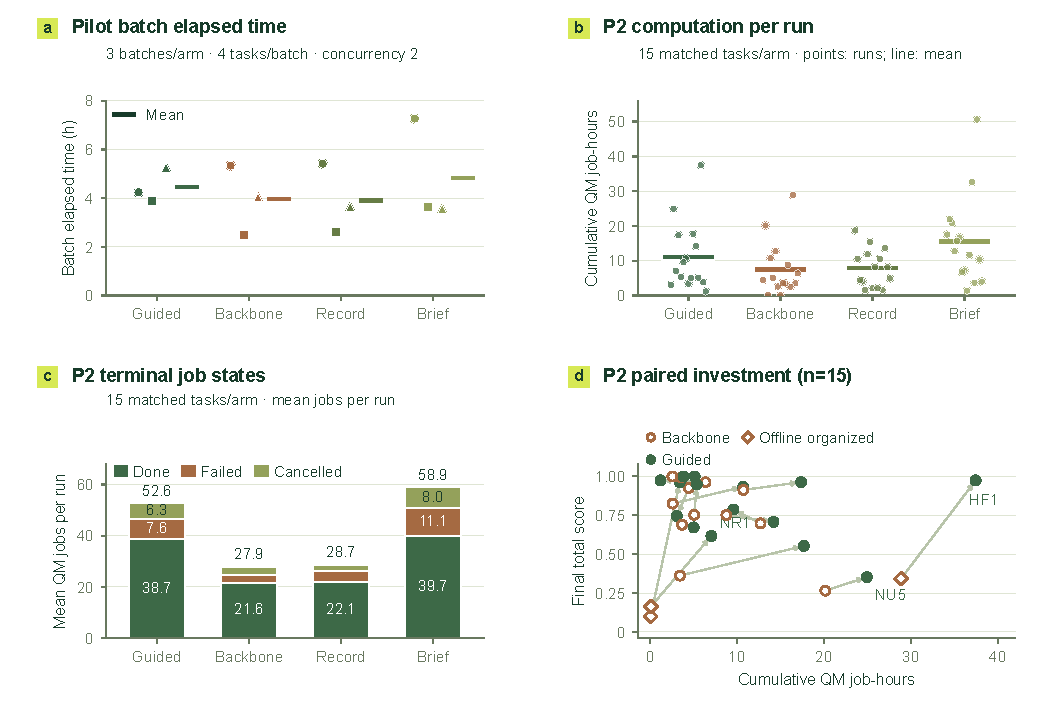
\includegraphics[width=\textwidth]{figures/bench_speed.pdf}
\caption{Research elapsed time and computational investment. (a) Twelve P1b four-task batches at concurrency two, three per arm; lines mark means. (b) Cumulative QM process durations for the 15 P2 tasks shared by all arms. (c) Mean completed, failed, and cancelled jobs in that cohort. (d) Same-task Backbone-to-Guided changes in investment and final score; diamonds mark offline-organized Backbone graphs. Job-hours sum process walltime; panel a measures batch latency. Backbone/M1 effort is reconstructed from native CPU time divided by four.}
\label{fig:bench-speed}
\end{minipage}
\end{figure*}

\begin{figure*}[p]
\begin{minipage}{\textwidth}
\centering
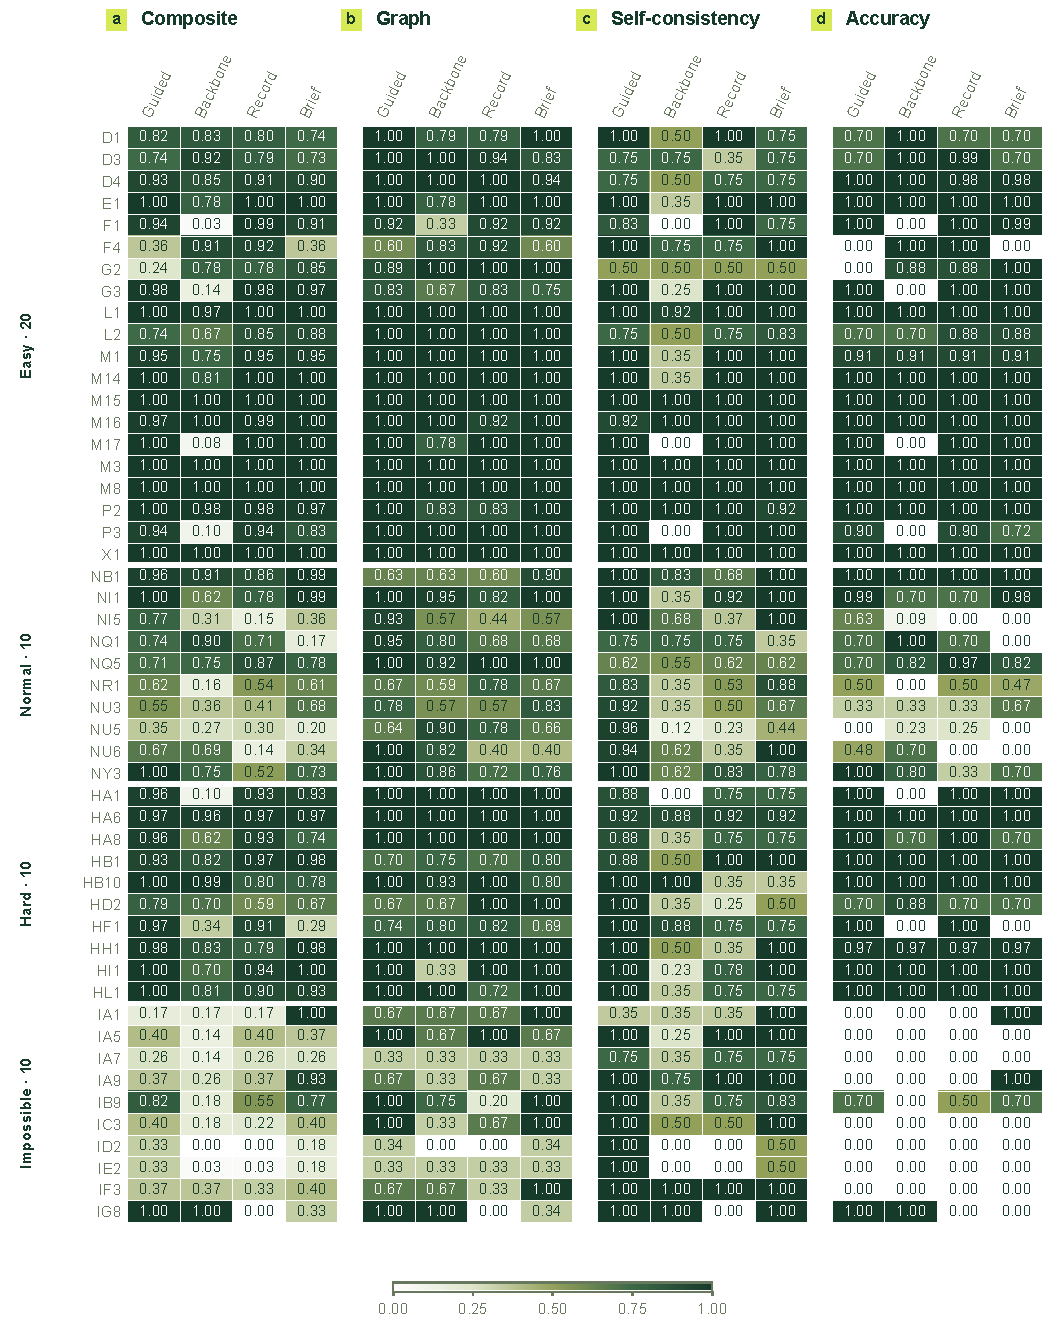
\includegraphics[width=\textwidth]{figures/bench_tasks_all.pdf}
\caption{Complete CloudraBench results for all 50 tasks and four configurations. The aligned blocks show composite, Graph, Self-consistency, and Accuracy on the same 0--1 scale; all 800 cells are present. Values are rounded to two decimals; the source table retains full precision.}
\label{fig:bench-tasks}
\vspace{6pt}
\end{minipage}
\end{figure*}

\begin{figure*}[!tbp]
\begin{minipage}{\textwidth}
\centering
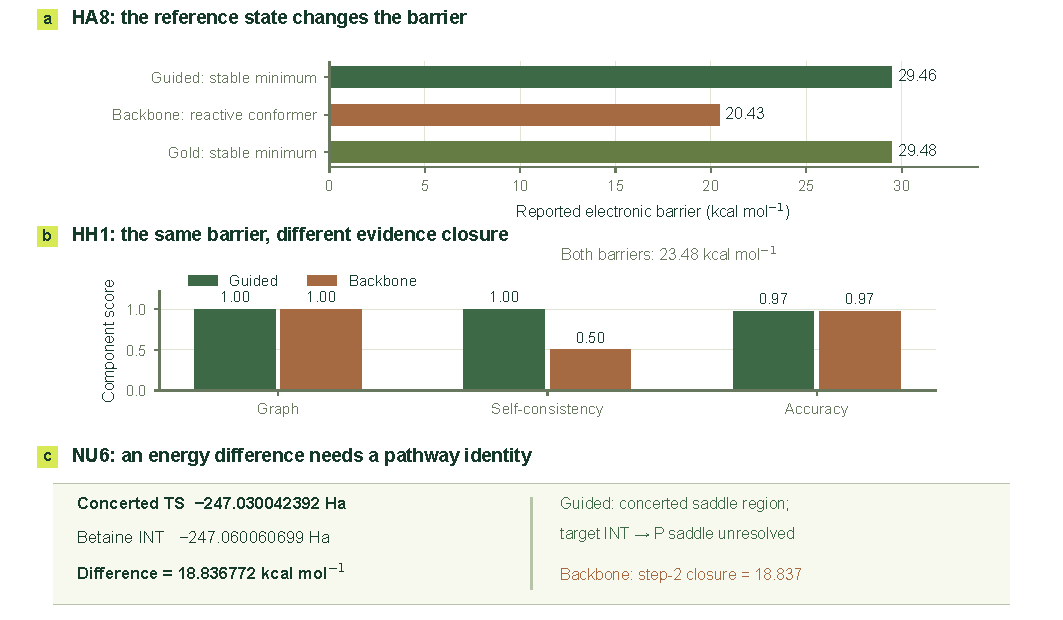
\includegraphics[width=\textwidth]{figures/bench_cases.pdf}
\caption{Scientific attribution in matched Guided--Backbone tasks. (a) HA8 barriers use stable-minimum or reactive-conformer references. (b) HH1 retains the same barrier and accuracy, with different evidence closure. (c) NU6's recorded energy difference is assigned to different pathways. Values and assignments derive from the archived records.}
\label{fig:bench-cases}
\end{minipage}
\end{figure*}

\begin{figure*}[!tbp]
\begin{minipage}{\textwidth}
\centering
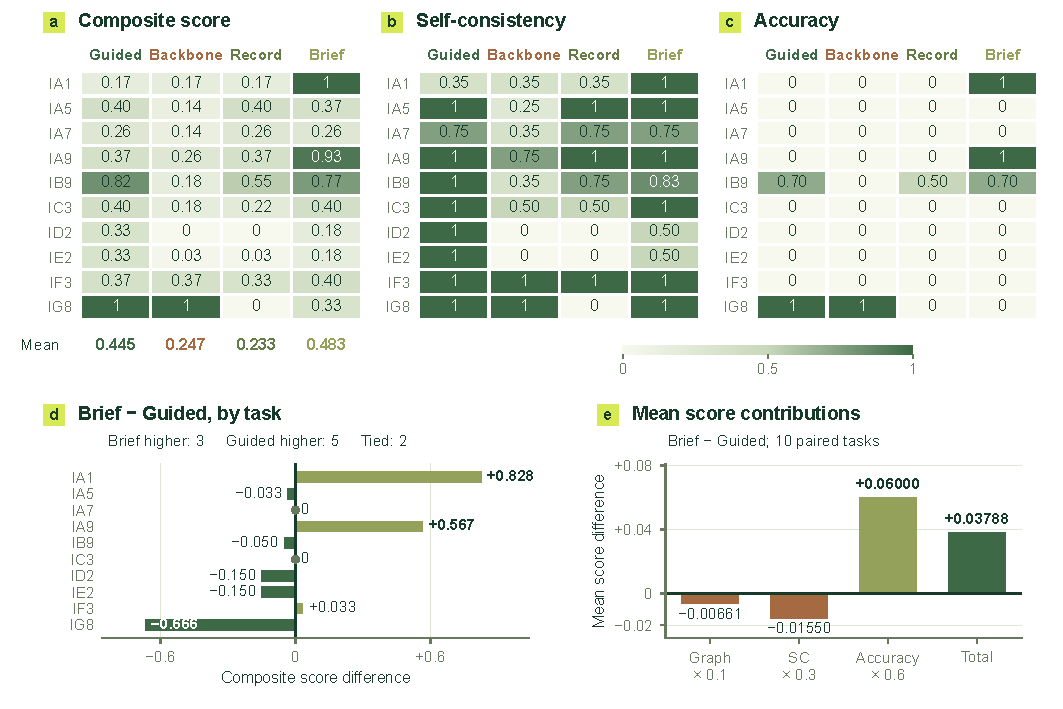
\includegraphics[width=\textwidth]{figures/bench_imp.pdf}
\caption{Impossible-tier outcomes and the brief-diagnostic ablation. (a--c) Composite, self-consistency (SC), and accuracy for all ten tasks and four arms, using the complete organized scores on a common 0--1 scale. Backbone denotes the actual same-backbone Standard arm. (d) Paired Brief-minus-Guided differences: the mean advantage of 0.03788 is concentrated in IA1 and IA9, with an opposite outcome in IG8; Guided scores higher on five tasks, Brief on three, and two tie. (e) The mean difference decomposes into weighted accuracy (+0.06000), Graph ($-0.00661$), and SC ($-0.01550$); the small discrepancy in their sum reflects rounding of saved totals. The paired task-bootstrap 95\% interval is $-0.188$ to +0.284; task-specific claims are analyzed below.}
\label{fig:bench-imp}
\end{minipage}
\end{figure*}

\begin{figure*}[!tbp]
\begin{minipage}{\textwidth}

\centering
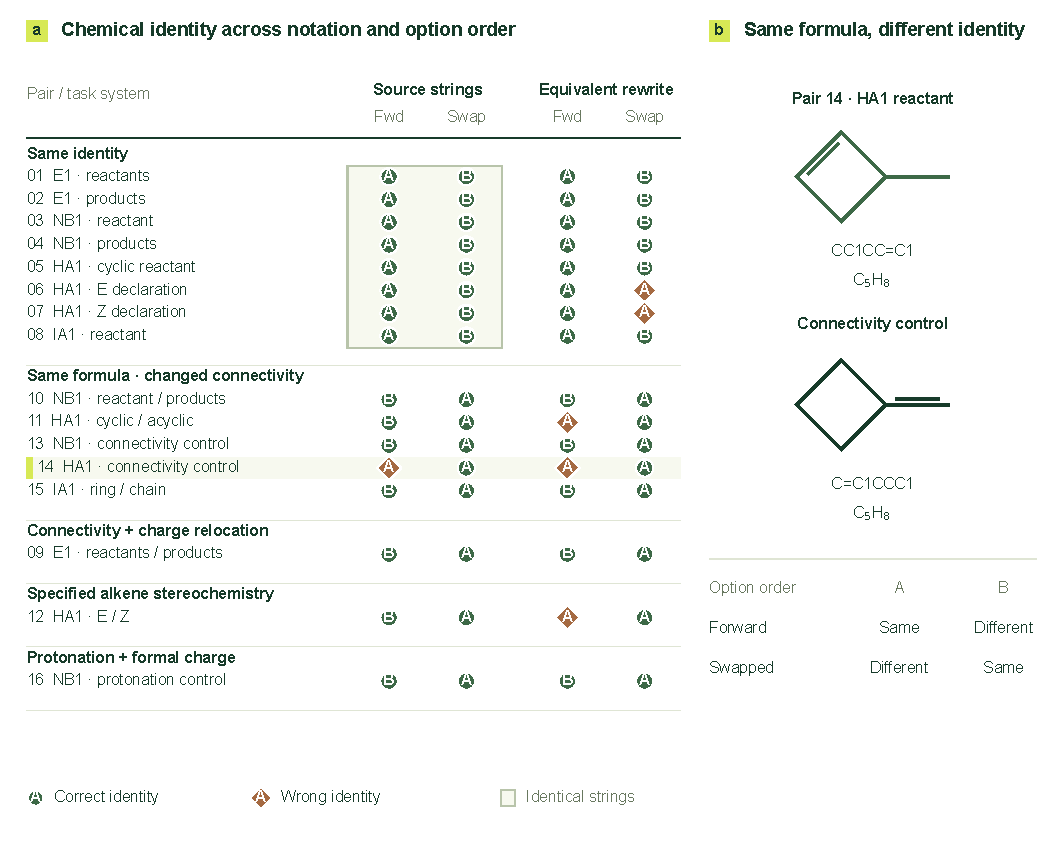
\includegraphics[width=\textwidth]{figures/fig06.pdf}
\caption{Molecular-identity judgments under changes in molecular representation and option order. Each of the 16 molecular pairs has four input conditions. Circles and diamonds indicate correct and incorrect judgments, respectively; the letters retain the model's actual answers. Shaded regions denote identical-string conditions. The right panel shows the pair-14 connectivities \texttt{CC1CC=C1} and \texttt{C=C1CCC1}, both C\textsubscript{5}H\textsubscript{8}, and the meanings of the answer options.}
\label{fig:06}
\end{minipage}
\end{figure*}

\begin{figure*}[!tbp]
\begin{minipage}{\textwidth}
\begin{minipage}[t]{.65\textwidth}
\vspace{0pt}
\centering
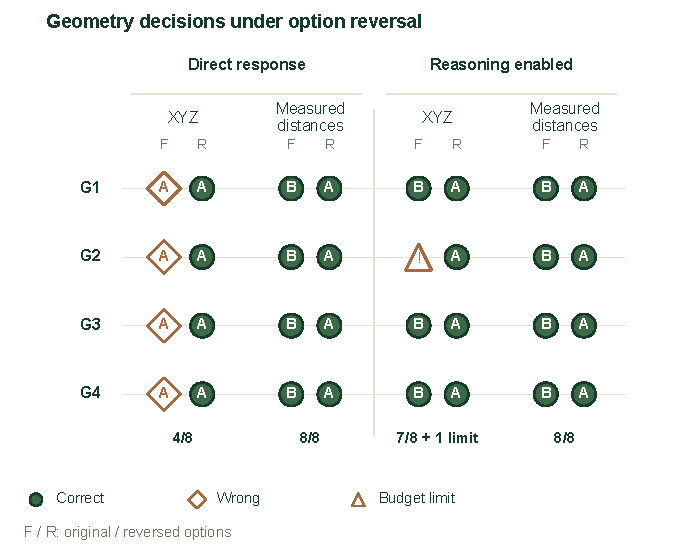
\includegraphics[width=\linewidth]{figures/fig07.pdf}
\caption{Geometry judgments under coordinate inputs and measured-distance inputs. Four source structures are compared under direct response and reasoning-enabled conditions, each with original (F) and reversed (R) option order. Circles indicate correct judgments, diamonds incorrect judgments, and the triangle a response that reached the output budget. Letters retain the actual answers.}
\label{fig:07}
\end{minipage}\hfill
\begin{minipage}[t]{.31\textwidth}
\vspace{0pt}
\centering
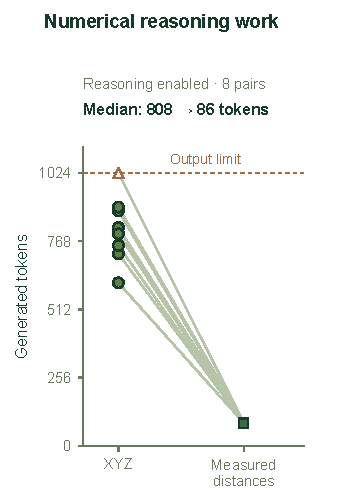
\includegraphics[width=\linewidth]{figures/fig08.pdf}
\caption{Generated-token counts with reasoning enabled. Each line connects Cartesian-coordinate input and measured-distance input for the same source structure and option order; eight paired comparisons are shown. The dashed line marks the output limit.}
\label{fig:08}
\end{minipage}
\end{minipage}
\end{figure*}

\begin{figure*}[!tbp]
\begin{minipage}{\textwidth}
\centering
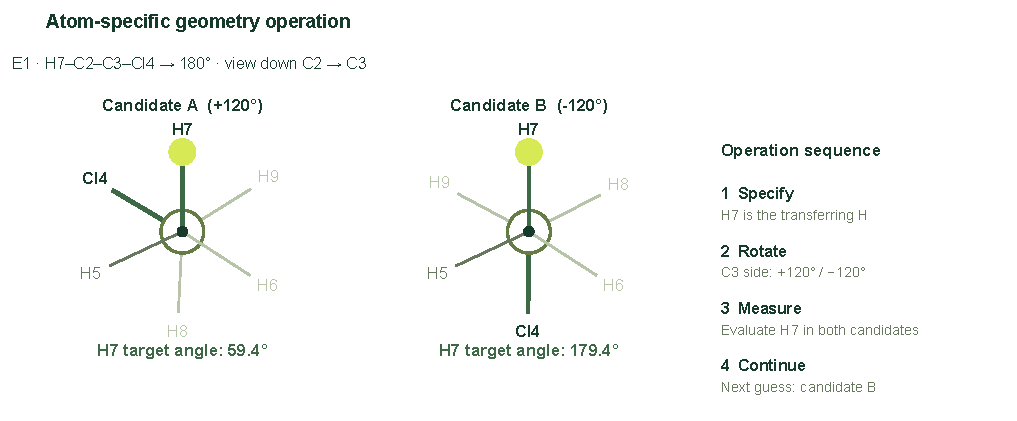
\includegraphics[width=.92\textwidth]{figures/fig09.pdf}
\caption{Target-specific geometry operations in E1. Newman projections retain the directions of the original candidate coordinates viewed down C2\(\to\)C3. H7 is the specified transferring atom. Candidate A and candidate B give target angles of 59.4° and 179.4°, respectively. The operation sequence is shown alongside the projections.}
\label{fig:09}
\vspace{5pt}
\begin{minipage}[t]{.48\textwidth}
\vspace{0pt}
\centering
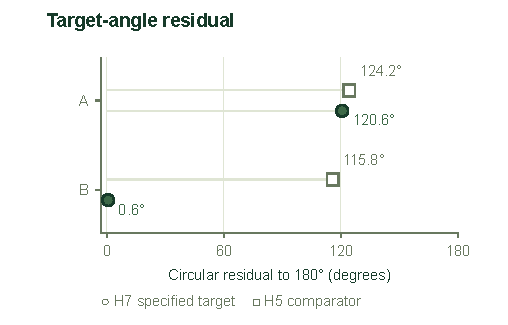
\includegraphics[width=\linewidth]{figures/fig10.pdf}
\caption{Circular angular residuals from the specified 180° target for candidates A and B. H7 is the specified target atom; H5 is the comparator.}
\label{fig:10}
\end{minipage}\hfill
\begin{minipage}[t]{.48\textwidth}
\vspace{0pt}
\centering
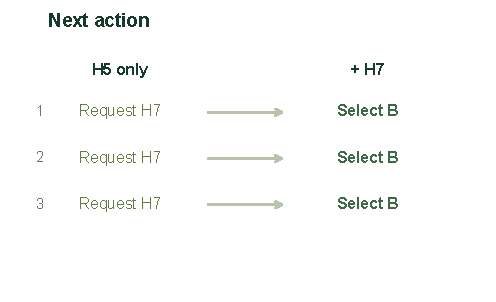
\includegraphics[width=\linewidth]{figures/fig11.pdf}
\caption{Next-action choices under three local option permutations. When only H5 measurements are supplied, the model requests H7 measurements; with H7 supplied, it selects candidate B.}
\label{fig:11}
\end{minipage}
\end{minipage}
\end{figure*}

\begin{figure*}[!tbp]
\begin{minipage}{\textwidth}
\centering
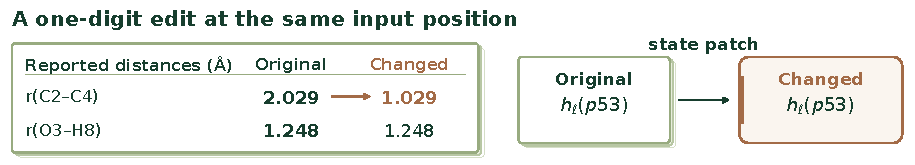
\includegraphics[width=.92\textwidth]{figures/fig12.pdf}
\caption{Intervention on a single reported distance. A one-digit edit changes the C2–C4 distance from 2.029 to 1.029 Å while O3–H8 remains 1.248 Å. The original-input residual state at token position 53 is inserted into the changed-input run at a specified layer. Token positions are zero-based.}
\label{fig:12}
\vspace{4pt}
\centering
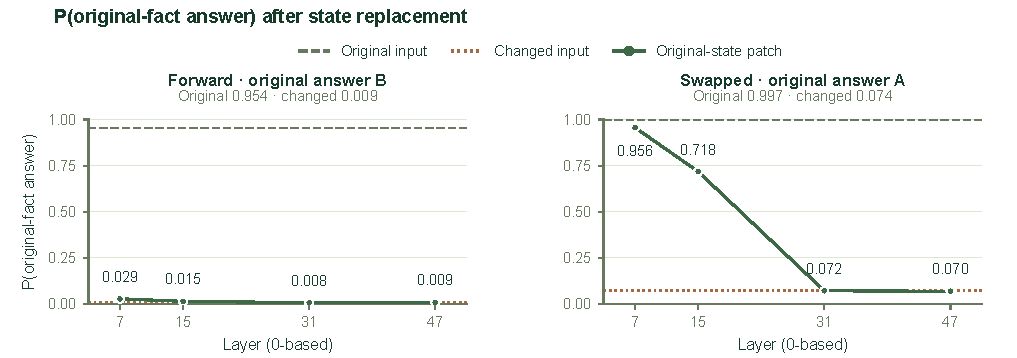
\includegraphics[width=.92\textwidth]{figures/fig13.pdf}
\caption{Original-fact answer probability after state replacement. Curves show full-vocabulary probability mass for the original-fact answer under forward (B) and swapped (A) option order, including bare and leading-space token spellings. Horizontal lines show original-input and changed-input baselines. Layer indices are zero-based.}
\label{fig:13}
\vspace{4pt}
\centering
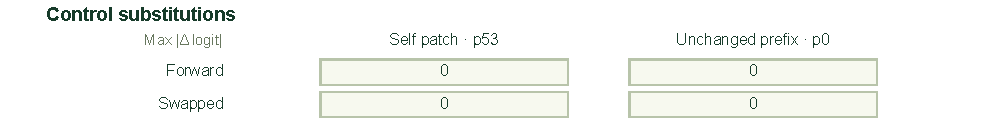
\includegraphics[width=.92\textwidth]{figures/fig14.pdf}
\caption{Control substitutions for the state-intervention experiment. Same-state self replacement at p53 and replacement of the unchanged prefix at p0 preserve all vocabulary logits in both option orders. The table reports the maximum absolute logit difference. Token positions are zero-based.}
\label{fig:14}
\end{minipage}
\end{figure*}

\begin{figure*}[!tbp]
\begin{minipage}{\textwidth}

\begin{minipage}[t]{.48\textwidth}
\vspace{0pt}
\centering
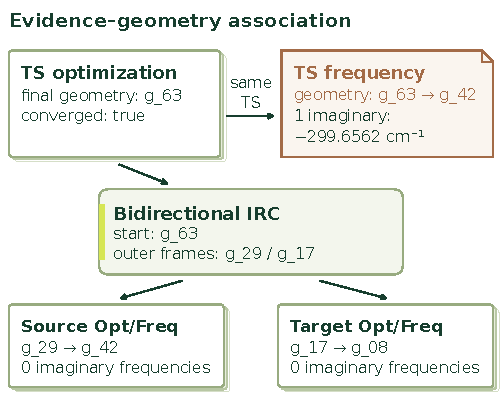
\includegraphics[width=\linewidth]{figures/fig15.pdf}
\caption{Evidence--geometry association in E1. The frequency geometry reference changes from g\_63 to g\_42 while local termination, convergence, energy, and frequency values remain fixed. Arrows retain the TS--IRC--endpoint optimization/frequency chain.}
\label{fig:15}
\end{minipage}\hfill
\begin{minipage}[t]{.48\textwidth}
\vspace{0pt}
\centering
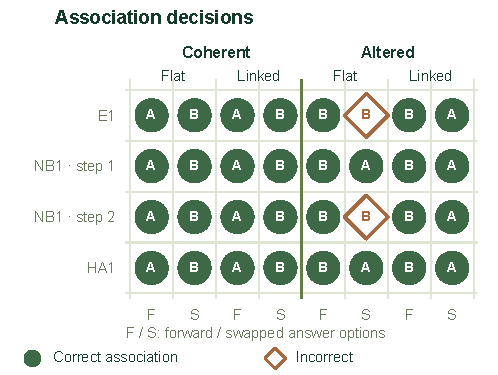
\includegraphics[width=\linewidth]{figures/fig16.pdf}
\caption{The 32 association judgments cross four source chains, coherent/altered links, flat/linked presentation, and forward/swapped answer order. Saved A/B responses and correctness markers are retained.}
\label{fig:16}
\end{minipage}
\end{minipage}
\end{figure*}

\begin{figure*}[!tbp]
\begin{minipage}{\textwidth}
\centering
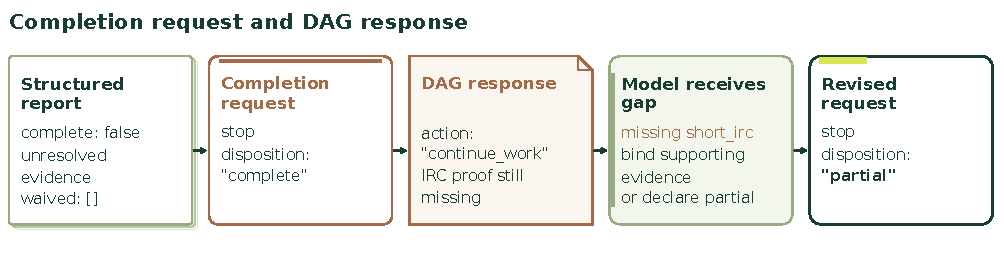
\includegraphics[width=.96\textwidth]{figures/fig17.pdf}
\caption{Completion requests and DAG feedback in the original IA1 trajectory. A report with unresolved evidence is followed by a completion request, a response identifying missing short\_irc proof, feedback to the model, and a revised partial-completion request.}
\label{fig:17}
\end{minipage}
\end{figure*}
